\chapter{Search by Snapを用いたユーザ実験}
\section{実験の目的}
  ?章で述べたように,慣れていない地域や周囲の文字が読めないに状況おいて,ユーザが目の前にある店舗の情報や条件に合致する店舗の情報を瞬時に取得することは容易ではない.
  位置情報を手がかりに周囲の検索を行い,条件に合った店舗が見つかったとしても,ユーザ自身が居る環境と検索行為とが分断されているため,そのその環境からその店舗を探す手間が残るという問題点がある.
  そのため,提案システムを用いることによって,位置情報を利用したサービスと比較して店舗を簡単かつ直感的に探索できることを確認する.
  本稿では,地域に慣れていないユーザを対象に評価を行う前段階として,提案システムのユーザビリティを評価するために,地元の大学生を対象にユーザ実験を実施する.

\section{実験の概要}
  実験は大阪府高槻市にある高槻本通りにおいて,昼間にユーザが飲食店を探している状況を想定して行った.
  実験参加者は情報系の学部に通う大学生10名である.

  実験参加者にはタスク(A)として,「小だるま JR高槻駅前店」,「肉丼専門店 高槻肉劇場」,「磯丸水産 高槻店」の3店舗について,使用できるクレジットカードの種類を``Visa'',``Mastercard'',``JCB'',``American Express'',``Diners Club''の5つのチェックボックスから全て選択すること,タスク(B)として,「おだいどこはなれ 高槻店」,「高槻ちゃぶちゃぶ」,「赤から 高槻店」の3店舗について,月曜日の営業開始時刻を数値で入力すること,の2点を課した.
  タスク(A)は図\ref{fig:exp_point}中\textcircled{\scriptsize 1}で示した位置に立った状態,タスク(B)は図\ref{fig:exp_point}中\textcircled{\scriptsize 2}で示した位置に立った状態で行った.
  実験に用いた携帯端末はクアンタ・コンピュータ社\footnote{http://www.quantatw.com}のVA-10J(Android 5.0.2)である.
  提案システムとの比較対象とする位置情報を用いたサービスは,ランキングやユーザの口コミ・写真をもとにレストランの検索が行えるサービスである食べログ\footnote{https://tabelog.com}を用いた.

\begin{figure}[tb]
  \begin{center}
    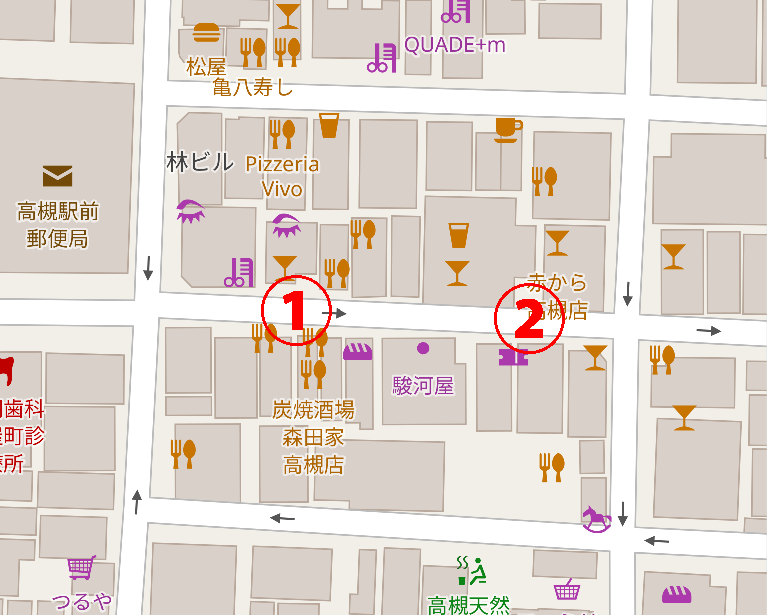
\includegraphics[clip, width=.95\columnwidth]{sbs_map_point.eps}
    \caption{実験の実施地点}
    \label{fig:exp_point}
  \end{center}
\end{figure}

\begin{figure}[t]
  \begin{minipage}{0.49\hsize}
    \begin{center}
      \includegraphics[clip, width=.95\textwidth]{sbs_interface.png}\\
      \caption{ユーザインタフェース}
      \label{fig:interface}
    \end{center}
  \end{minipage}
  \begin{minipage}{0.49\hsize}
    \begin{center}
      \includegraphics[clip, width=.95\textwidth]{sbs_exp_scenery.jpg}\\
      \caption{実験の風景}
      \label{fig:exp_scenery}
    \end{center}
  \end{minipage}
\end{figure}

\section{実験の手順}
  初めに,提案システムと食べログの使い方を実験参加者に説明する.
  次に,実験参加者に回答用フォームのURLを伝え,参加者は自身のスマートフォンでフォームを開く.
  実験に用いるシステムを起動した状態で参加者に実験用のスマートフォンを渡す.
  実験参加者はシステムを用いて求められている情報を探索し,フォームに入力して送信する.
  実験参加者がシステムの操作を始めてから送信ボタンをタップするまでの時間を計測する.
  実験の風景を図\ref{fig:exp_scenery}に示す.

  実験参加者をグループ(1)とグループ(2)に2分割し,グループ(1)にはタスク(A)を提案システム,タスク(B)を食べログを用いて行うよう指示を出し,グループ(2)にはタスク(A)を食べログ,タスク(B)を提案システムを用いて行うよう指示を出した.
  実験終了後には,参加者に「求めていた情報の見つけやすさ(簡便性)」,「情報探索の直感性(直感性)」について,食べログと提案システムとの間で5段階評価のアンケートへの回答を求めた.

\section{実験の結果}
  実験参加者がシステムに操作を初めてから指示された情報を全て収集し,送信ボタンをタップするまでの時間を計測し,タスク(A)とタスク(B)に関して提案システムを用いた場合と食べログを用いた場合とにおいて,探索時間の平均値を比較した.その結果を図\ref{fig:result_time}に示す.
  タスク(A)において,提案手法を用いた場合の探索時間は食べログを用いた場合よりも有意に短い($t(8)=2.343, p<.05$)ことが確認された.
  タスク(B)においても,提案手法を用いた場合の探索時間は食べログを用いた場合よりも有意に短い($t(8)=4.370, p<.05$)ことが確認された.

  各タスクにおいて,ユーザが正確に情報を収集できたかを測定するために,対象とした3店舗のうち,正確に情報を取得できた店舗数の割合を正解率として測定し,提案システムを用いた場合と食べログを用いた場合とにおいて,正解率の平均値を比較した.その結果を図\ref{fig:result_acc}に示す.
  タスク(A)において,提案手法を用いた場合と食べログを用いた場合とで,正解率に有意差は見られなかった($t(8)=1.000, n.s.$).
  タスク(B)においても,提案手法を用いた場合と食べログを用いた場合とで,正解率に有意差は見られなかった($t(8)=1.633, n.s.$).

  情報探索の簡便性と直感性について5段階のリッカート尺度を用い,「1」を「食べログ」,「5」を「提案システム」として5段階で回答してもらった.
  そのアンケート結果の分布を図\ref{fig:result_question}に示す.
  簡便性に関する平均値は4.4,直感性に関する平均値は4.5であった.

  \begin{figure}[tb]
    \begin{center}
      \includegraphics[clip, width=.95\columnwidth]{sbs_result_time.pdf}
      \caption{探索時間}
      \label{fig:result_time}
    \end{center}
  \end{figure}
  \begin{figure}[tb]
    \begin{center}
      \includegraphics[clip, width=.95\columnwidth]{sbs_result_acc.pdf}
      \caption{正解率}
      \label{fig:result_acc}
    \end{center}
  \end{figure}
  \begin{figure}[tb]
    \begin{center}
      \includegraphics[clip, width=.95\columnwidth]{sbs_result_question.pdf}
      \caption{アンケート(1: 食べログ〜 5: 提案システム)}
      \label{fig:result_question}
    \end{center}
  \end{figure}

\section{議論}
\label{sec:discussion}
\subsection{実験結果に関して}
  実験結果から,情報探索時間に関しては,本稿で扱ったいずれの場合においても,提案システムを用いた場合は食べログを用いた場合よりも探索時間が有意に短くなることが明らかとなった.このことから,提案システムを用いることによって,位置情報のみを用いた場合と比較してユーザはより素早く求めている情報を取得することが可能になるといえる.
  情報探索の正確さに関しては,本稿で扱ったいずれの場合においても,提案システムを用いた場合と食べログを用いた場合とでは正解率に有意差は見られなかった.このことから,言語障壁がなければ位置情報のみを用いても正確に情報を探索することが可能であり,提案システムを用いた場合においても正確な情報探索が可能であるといえる.
  また,アンケート結果から,提案システムを用いることによって,位置情報のみを用いた場合と比較してより簡単かつ直感的に情報が探索できるようになることが示唆された.

\subsection{提案システムで達成されたこと}
  提案システムを用いることによって,本研究の目的である,ユーザの目の前にある店舗の情報を直感的かつ簡単に取得できることが達成されたと考えられる.
  これにより,?章で述べた,慣れていない地域においても,ユーザが求める条件に合致する店舗を探索できるようになることが示唆された.

\subsection{課題}
\label{sec:limitation}
  本研究の課題として,(1)OSMのノードと看板画像を手作業で関連付けなければならない点,(2)インターネット上の情報から多種多様な店舗の看板画像を大量に集めることは困難であるため,手作業で看板画像を1店舗につき100枚程度集めなければならない点,が挙げられる.
  (1)に対しては,看板画像を提示してユーザに店舗名を回答するシステムを実装することで解決でき,(2)に対してはユーザに店舗の看板画像を提示し,それと同じ写真を撮影して投稿するシステムを実装することで解決できると考えられる.
  これらのシステムにゲーミフィケーションを利用し,ユーザの行動に対して報酬を与えることによって,多数のデータを効率よく収集できると考えられる.

\subsection{今後の展望}
  今後の展望として,看板認識をサーバ上で行うのではなく,Tiny--YOLO等を用いて携帯端末上で行うことを検討する.これにより,サーバへ画像を送信する必要がなくなるため,通信量の大幅な軽減が期待される.
  また,OSMのデータは誰もが編集可能であるため,\ref{sec:limitation}節で述べたように,その地域に慣れている地元のユーザが自身でデータを収集し,OSMを通して活用できるようになる枠組みの構築を目指す.
  OSMのノードには``cuisine''タグが存在し,``burger'',``noodle'',``japanese'',``chinese''など,飲食店で提供される食品の種類を表す値を追加できる.他にもベジタリアン向けのメニューが提供されていることを表す``diet:vegetarian''や,イスラム教の戒律で許されている食品のみを使用したメニューが提供されていることを表す``diet:halal''などのタグも存在する.
  さらに,店舗名の英語またはローマ字表記を表す``name:en''タグや中国語表記の``name:zh''タグ,韓国語表記の``name:ko''タグなどを充実させることによって,ユーザインタフェースを多言語に対応させることが可能となる.
  これらのデータを活用することにより,その地域に慣れていない人や,地元の文字が読めない外国人観光客に対して,求めている情報を容易に取得でき,アレルギーや宗教的制約などの理由による食事制限にも対応可能なナビゲーションを実現できる.
  
  本稿における実験参加者は地元の大学生であるため,地域に慣れていないユーザや非漢字圏など地元の文字が読めないユーザを対象としたユーザ実験を実施する.
